% XeLaTeX -> BibTeX -> XeLaTeX -> XeLaTeX
\documentclass[aspectratio=169,11pt]{beamer}
\usepackage[UTF8,fontset=fandol]{ctex}
\usepackage{amsmath,amssymb,bm,booktabs,tabularx,array,graphicx,listings,xurl}
\usepackage[numbers,square,sort&compress]{natbib}
\usetheme{Madrid}
\usecolortheme{default}
\setbeamertemplate{navigation symbols}{}
\setbeamertemplate{bibliography item}[text]
\hypersetup{colorlinks=true,linkcolor=.,citecolor=blue,urlcolor=blue,pdftitle={TableLab：基于本地字段检索的中文表格问答与预测},pdfauthor={郑嘉诚}}
\newcommand{\code}[1]{\nolinkurl{#1}}
\newcommand{\smallnote}[1]{\par\vspace{1.5mm}{\scriptsize #1\par}}
\newcommand{\Train}{\mathcal T}\newcommand{\Valid}{\mathcal V}
\newcolumntype{Y}{>{\raggedright\arraybackslash}X}
\lstset{basicstyle=\ttfamily\footnotesize,breaklines=true,columns=fullflexible,keepspaces=true,showstringspaces=false}
\title[TableLab]{TableLab：基于本地字段检索的\\中文表格问答与预测}
\subtitle{天津大学机器学习与人工智能课程报告}
\author[郑嘉诚]{\href{https://karcen.github.io/}{郑嘉诚}}
\institute[马寅初经济学院]{马寅初经济学院\quad 应用经济学\\学号：2026209004}
\date[2026.11.01]{\today}
\begin{document}
\begin{frame}[plain]
\titlepage
\end{frame}

\section{研究问题与数据}
\begin{frame}{字段检索和模型预测分别检查}
用户问“CollgCr 社区的平均成交价是多少”，程序需要先选对社区与成交价两列，再筛选记录并求均值。
\par\medskip
本文分别检查两件事：检索器把所需字段排在什么位置；使用相同样本时，输入变量和算法怎样影响预测误差。
\par\medskip
选错列后，算术结果仍可能正确。因此字段检索和模型预测分别报告。
\smallnote{TaPas 从表中选择单元格并聚合\citep{herzig2020}；TableLab 检索字段说明，再读取原表计算\citep{lewis2020}。}
\end{frame}

\begin{frame}{四份数据与预测输入}
\small
\begin{tabularx}{\textwidth}{llY}
\toprule
数据 & 预测目标 & 输入变量\\\midrule
房价，1,460 条 & 成交价 & 整体质量、居住面积、建成年份、地下室面积、车位数、社区\\
Adult，48,842 条 & 年收入是否超过 5 万美元 & 年龄、教育编码、周工时、用工类别、职业、婚姻状况\\
NBA，12,844 条 & 场均得分 & 年龄、身高、体重、选秀年份类别\\
学生，1,000 条 & 数学成绩 & 性别、父母教育程度、午餐类别、是否完成备考课程\\\bottomrule
\end{tabularx}
\par\medskip\normalsize
四份表分别分析。学生成绩按考前预测处理，输入中不含同期阅读和写作成绩。
\smallnote{Adult 行数包含独立测试文件的 16,281 条记录，该文件未参加模型拟合或验证。数据来源见\citep{house,adult,nba,student}。}
\end{frame}

\begin{frame}{原单次划分复核的样本}
\small
\begin{tabularx}{\textwidth}{lrrY}
\toprule
主题 & 训练 & 验证 & 划分\\\midrule
房价 & 1,168 & 292 & 固定随机 80/20。\\
Adult & 26,049 & 6,512 & 在原训练文件内按收入分层，相同预测字段的记录放在同组。\\
NBA & 9,561 & 3,283 & 后六个完整赛季留出。\\
学生 & 800 & 200 & 固定随机 80/20。\\\bottomrule
\end{tabularx}\par
\par\medskip\normalsize
同一任务的两个算法使用相同记录。Adult 只采用五折分组器的第一个划分；学生输入不包含同期其他考试分数。
\smallnote{主实验使用四份数据各两个模型；房价与 NBA 另有四个改变划分方式的配置。}
\end{frame}

\section{字段检索与统计计算}
\begin{frame}{先检索字段说明，再计算均价}
\begin{tabularx}{\textwidth}{lY}
\toprule
收到的问题 & “CollgCr 社区的平均成交价是多少？”\\
本地检索 & 查找社区、成交价的字段说明与均值计算说明。\\
方案生成 & DeepSeek API 返回字段名、筛选条件和统计方法。\\
程序执行 & 读取完整筛选样本，计算均值，保存结果。\\
\bottomrule
\end{tabularx}\par
\par\medskip
本地字段检索为 DeepSeek 提供说明；返回的 JSON 方案经核对后，由本机读取原表计算成交均价。
\smallnote{检索增强生成的基本思路见 \citet{lewis2020}。本项目检索本地字段说明。}
\end{frame}

\begin{frame}{计算 CollgCr 社区的平均成交价}
\begin{columns}[T,onlytextwidth]
\begin{column}{.49\textwidth}
表格中的两列：
\par\medskip
\code{Neighborhood}：社区类别。
\par\medskip
\code{SalePrice}：成交价。
\par\medskip
选出社区等于 CollgCr、成交价有记录的行。
\end{column}
\begin{column}{.47\textwidth}
成交记录的计算结果为
\[
n=150,\quad \sum y_i=29\,694\,866.
\]
\[
\bar y=\frac{29\,694\,866}{150}
\]
\centering\large 197,965.77 美元
\end{column}
\end{columns}
\smallnote{计算记录：\code{tables/teaching/collgcr_members.csv}。完整房价表有 1,460 条记录。}
\end{frame}

\begin{frame}[fragile]{把问题写成计算参数}
\begin{lstlisting}
{
  "dataset": "house",
  "operation": "aggregate",
  "columns": ["SalePrice"],
  "filters": [
    {"column": "Neighborhood", "op": "eq", "value": "CollgCr"}
  ],
  "group_by": [],
  "metric": "mean"
}
\end{lstlisting}
每个参数都能与原问题核对：哪个表、哪一列、筛选谁、算什么。
\smallnote{本例使用人工给定并已执行的参数。}
\end{frame}

\begin{frame}{把字符片段转成 TF--IDF 权重}
“平均成交价”拆成长度为 2、3、4 的连续字符片段。设片段 $t$ 在说明 $d$ 中出现 $c_{td}$ 次。
\[
\operatorname{tf}(t,d)=1+\log c_{td}\quad(c_{td}>0),
\]
\[
\operatorname{idf}(t)=1+\log\frac{N+1}{\operatorname{df}(t)+1}.
\]
TF 对重复计数取对数；IDF 增加较少见片段的权重。权重为二者之积。
\smallnote{当前程序使用字符 2--4 元组、平滑 IDF 与次线性 TF，见 \citet{sklearntfidf}。}
\end{frame}

\begin{frame}{用余弦相似度排序字段说明}
权重向量先归一化，查询与文档的点积就是余弦相似度：
\[
s(q,d)=\frac{\mathbf w_q^{\mathsf T}\mathbf w_d}{\|\mathbf w_q\|_2\|\mathbf w_d\|_2}.
\]
\begin{tabularx}{\textwidth}{Yr}
\toprule
开头均价问题的实际检索 & 分数\\\midrule
\code{Neighborhood} 字段说明 & 0.176436\\
\code{SalePrice} 字段说明 & 0.070664\\
房价数据说明 & 0.058073\\\bottomrule
\end{tabularx}\par
\smallnote{房价索引共 90 份文档，最多返回六条正相似度结果。分数衡量问题与说明之间的词面匹配。}
\end{frame}

\begin{frame}{16 道固定检索题的目标都在前六位}
四份数据各有 4 道题，每题指定一条目标字段或方法说明。
\par\medskip
\begin{tabularx}{\textwidth}{Yr}
\toprule
目标说明的排名 & 题数\\\midrule
第一位 & 15\\
第二位 & 1\\
前六位命中 & 16\\\bottomrule
\end{tabularx}
\[
\operatorname{MRR}=\frac{15+1/2}{16}=0.96875.
\]
\smallnote{15 道题写出了目标英文字段名。排在第二位的题目询问 \code{player_name} 是否是唯一身份，姓名说明排在身高说明之后。}
\end{frame}

\section{原固定参数实验}
\begin{frame}{预测模型使用相同的输入和划分}
\begin{tabularx}{\textwidth}{lY}
\toprule
模型 & 预测方法\\\midrule
均值基线 & 连续目标都预测为训练均值，用作误差参照。\\
线性回归 & 用处理后的特征拟合 $\hat y_i=\beta_0+z_i^{\mathsf T}\beta$。\\
逻辑回归 & 用 $p_i=1/(1+e^{-\eta_i})$ 预测高收入概率，阈值为 0.5。\\
随机森林 & 平均 120 棵树的预测；最大深度 12，叶节点至少 5 条记录。\\\bottomrule
\end{tabularx}
\par\medskip
先划分样本，再用训练集确定插补、缩放和类别编码。实验固定超参数。
\smallnote{逻辑回归使用 $C=1$ 和 L-BFGS，最多迭代 1,500 次。模型定义见\citep{sklearn,breiman2001}，详细推导放在补充页。}
\end{frame}

\begin{frame}{用 MAE、RMSE 和 $R^2$ 评价预测}
记验证残差 $e_i=y_i-\hat y_i$，验证数为 $n_V$。
\[
\operatorname{MAE}=\frac1{n_V}\sum_i|e_i|,\qquad
\operatorname{RMSE}=\sqrt{\frac1{n_V}\sum_i e_i^2}.
\]
MAE 平均绝对差；RMSE 对大误差更敏感，二者保留目标原单位。
\[
R^2=1-\frac{\sum_i e_i^2}{\sum_i(y_i-\bar y_V)^2}.
\]
$R^2$ 分母使用验证均值衡量波动。可执行的常数预测仍使用训练均值。
\end{frame}

\begin{frame}{房价误差同时取决于输入变量和算法}
\small
\begin{tabularx}{\textwidth}{Yrr}
\toprule
输入变量 & 线性回归 RMSE & 森林 RMSE\\\midrule
面积、整体质量 & 44,159.60 & 39,205.81\\
再加建成年份、地下室面积、车位数和社区 & 36,461.68 & 33,611.50\\\bottomrule
\end{tabularx}
\par\medskip\normalsize
两组模型使用相同的 1,168 条训练记录和 292 条验证记录。加入四个变量后，两种算法的误差都下降。
\par\medskip
六变量线性回归比两变量森林的 RMSE 低约 2,744 美元。
\smallnote{单位为美元。两字段结果来自演示计算，六字段结果来自固定基准实验。四个变量同时加入，表中反映其共同变化。}
\end{frame}

\begin{frame}{房价预测中森林的误差较小}
\begin{center}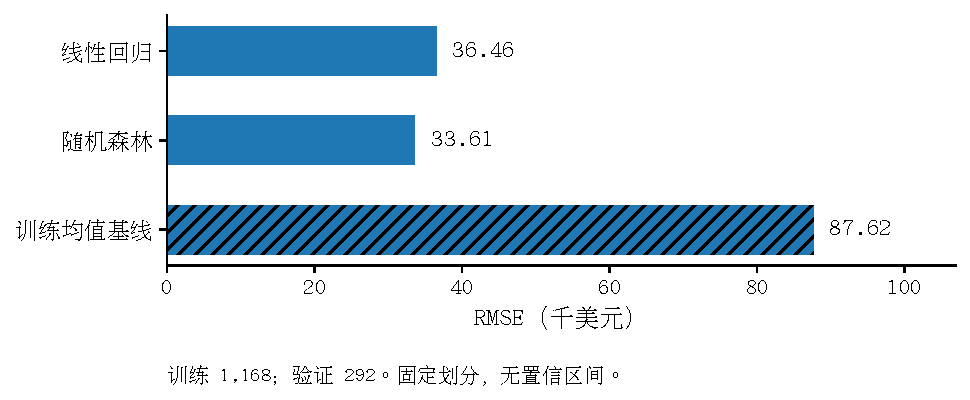
\includegraphics[width=.78\textwidth,height=.62\textheight,keepaspectratio]{figures/house_rmse_slide.pdf}\end{center}
\small
线性回归 $R^2=0.8267$，森林 $R^2=0.8527$。六个输入变量相同；线性回归与森林的 MAE 分别为 22,339.33 和 20,019.09 美元。
\smallnote{训练 1,168，验证 292；误差来自同一固定划分。}
\end{frame}

\begin{frame}{收入分类的 ROC 曲线}
\begin{center}
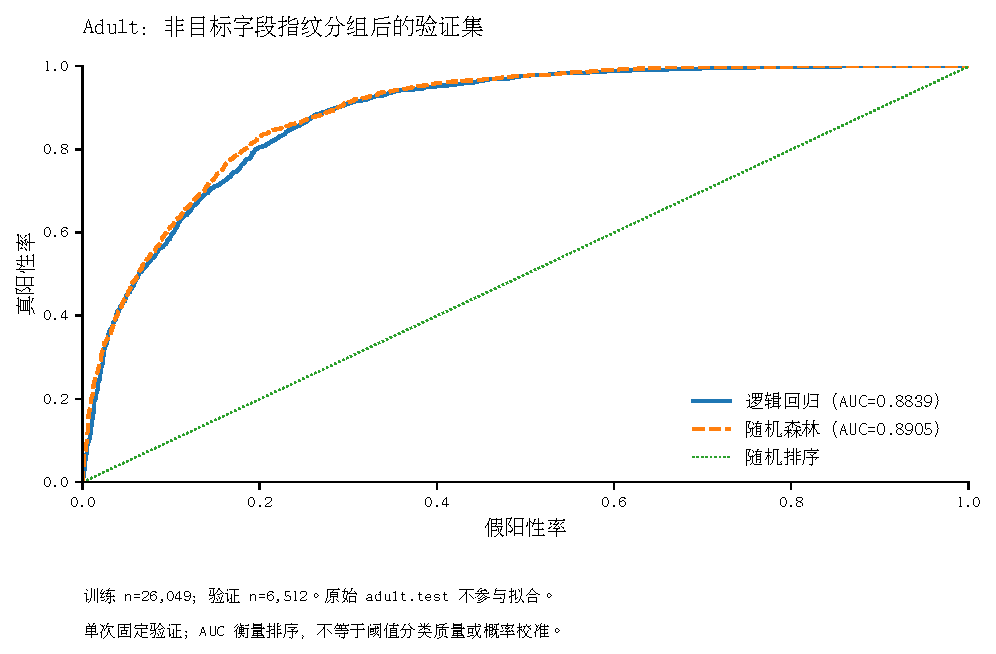
\includegraphics[trim=0 49bp 0 21bp,clip,width=.76\textwidth,height=.63\textheight,keepaspectratio]{figures/adult_roc.pdf}
\end{center}
\small
曲线比较不同阈值下的识别与误报比例。森林 AUC 为 0.8905，逻辑回归为 0.8839。
\smallnote{验证记录共 6,512 条，含 1,568 个正例。AUC 比较正负记录的排序，并列分数计作一半。}
\end{frame}

\begin{frame}{收入分类中森林的 AUC 更高、F1 更低}
\begin{center}\small
\begin{tabular}{lrrrr}
\toprule
模型 & AUC & F1 & Brier & 对数损失\\\midrule
逻辑回归 & 0.8839 & 0.6026 & 0.1150 & 0.3559\\
随机森林 & 0.8905 & 0.5916 & 0.1125 & 0.3484\\\bottomrule
\end{tabular}\par
\end{center}
森林识别 791 个正例，误报 315 个，漏报 777 个；逻辑回归分别为 849、401 和 719 个。
\par\medskip
AUC 比较正负记录的整体排序；F1 取决于阈值后的分类。森林减少误报，同时漏掉更多正例。
\smallnote{阈值均为 0.5；原始 adult.test 未参加性能计算。}
\end{frame}

\begin{frame}{用身体属性和选秀年份预测得分}
\begin{center}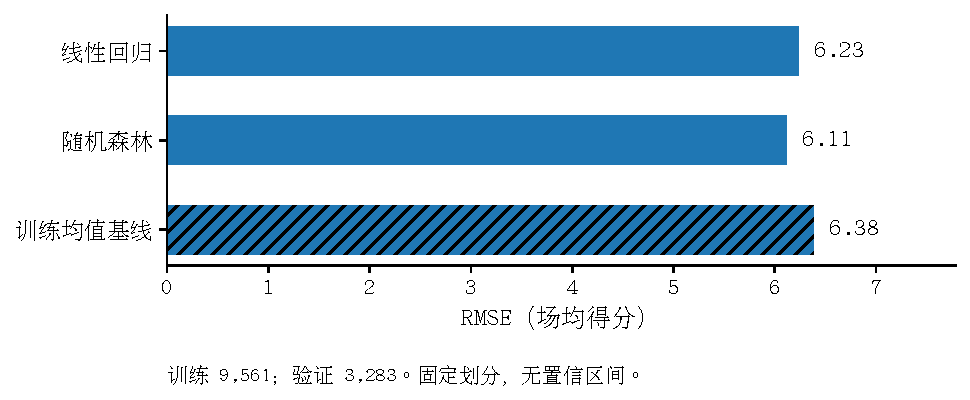
\includegraphics[width=.78\textwidth,height=.62\textheight,keepaspectratio]{figures/nba_rmse_slide.pdf}\end{center}
\small
输入为年龄、身高、体重和选秀年份。线性回归 $R^2=0.0390$，森林为 0.0753。
\smallnote{验证为 2017--18 至 2022--23。森林 RMSE 为 6.112 分，训练均值基线为 6.380 分，相差约 0.27 分。}
\end{frame}

\begin{frame}{学生成绩预测中线性回归的误差略低}
\begin{center}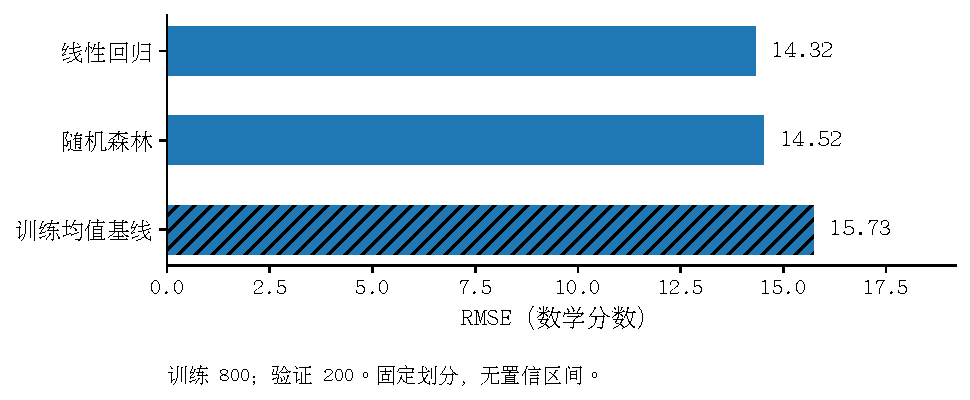
\includegraphics[width=.78\textwidth,height=.62\textheight,keepaspectratio]{figures/students_rmse_slide.pdf}\end{center}
\small
输入性别、父母教育、午餐类别和备考课程。线性回归 $R^2=0.1573$，森林为 0.1331。
\smallnote{训练 800、验证 200。线性回归 RMSE 比森林低 0.204 分；备考课程系数描述样本关联。}
\end{frame}

\begin{frame}{换一种划分，评价的问题也变了}
\small
\begin{tabularx}{\textwidth}{Yrr}
\toprule
划分 & 线性回归 RMSE & 森林 RMSE\\\midrule
房价：2010 年 175 条记录留出 & 35,008.88 & 30,310.72\\
NBA：姓名分组，验证 2,472 条 & 5.835 & 6.016\\\bottomrule
\end{tabularx}\par
\par\medskip\normalsize
房价按年份留出，NBA 按姓名分组。每一行使用相同验证记录比较两个算法，误差按各自目标的单位报告。
\smallnote{房价单位为美元；NBA 为场均得分。NBA 姓名分组的训练集为 10,372 条，验证集为 2,472 条；同名球员身份待核实。}
\end{frame}

\section{多模型与参数搜索}
\begin{frame}{四个任务都做多模型、调参与解释}
比较常数、线性正则化、决策树、森林、Extra Trees、提升树与近邻，共九种预设方法。\par\medskip
森林与提升树分别增加网格、TPE 两条流程。每个任务共十三条比较流程，使用相同输入字段。\par\medskip
训练与验证曲线检查拟合差距；SHAP 解释字段贡献，删去特征组后重新调参检验替代信息。\par\medskip
此前为单次划分，森林用 120 棵树；此处为三折嵌套，预设森林用 64 棵树。样本也不同，两组数值不能当作调参前后的变化。
\end{frame}

\begin{frame}{外层评价，内层选参数}
\begin{tabularx}{\textwidth}{lY}\toprule
任务 & 内外层划分约束\\\midrule
房价、学生 & 固定随机三折。\\
Adult & 按原始非目标字段指纹分组并分层。\\
NBA & 按完整赛季向前滚动，验证晚于训练。\\\bottomrule\end{tabularx}
\par\medskip
外层三折，内层沿用同一分折规则再分三折；每次搜索十二组参数。插补、缩放和编码均在训练折内拟合。\smallnote{两种搜索使用相同十二点离散域。主搜索共 1,728 次内层拟合，消融另行搜索。}
\end{frame}

\begin{frame}{房价的多模型比较}
\begin{center}\includegraphics[width=.92\textwidth,height=.72\textheight,keepaspectratio]{figures/research/benchmark_house_slide.pdf}\end{center}
\small 提升树＋网格的三折平均 RMSE为 32338.23。\smallnote{点为各折，误差线为折间标准差；排序描述本次结果。}
\end{frame}

\begin{frame}{收入分类的多模型比较}
\begin{center}\includegraphics[width=.92\textwidth,height=.72\textheight,keepaspectratio]{figures/research/benchmark_adult_slide.pdf}\end{center}
\small 提升树＋网格的三折平均 AUC为 0.8913。\smallnote{点为各折，误差线为折间标准差；排序描述本次结果。}
\end{frame}

\begin{frame}{NBA 得分的多模型比较}
\begin{center}\includegraphics[width=.92\textwidth,height=.72\textheight,keepaspectratio]{figures/research/benchmark_nba_slide.pdf}\end{center}
\small 随机森林的三折平均 RMSE为 5.698。\smallnote{点为各折，误差线为折间标准差；排序描述本次结果。Elastic Net 在三折中系数全为零，等于训练均值基线。}
\end{frame}

\begin{frame}{学生成绩的多模型比较}
\begin{center}\includegraphics[width=.92\textwidth,height=.72\textheight,keepaspectratio]{figures/research/benchmark_students_slide.pdf}\end{center}
\small Ridge的三折平均 RMSE为 13.545。\smallnote{点为各折，误差线为折间标准差；排序描述本次结果。Elastic Net 在三折中系数全为零，等于训练均值基线。}
\end{frame}

\begin{frame}{调参收益要在外层验证}
\begin{center}\includegraphics[width=.92\textwidth,height=.64\textheight,keepaspectratio]{figures/research/search_slide.pdf}\end{center}
{\footnotesize 外层变化（提升树）：房价 RMSE 降 966.57 美元，NBA 降 0.014 分；学生降 0.115 / 0.082 分，收入 AUC 增 0.0001。森林在收入和 NBA 上反而略差。\par}\smallnote{学生依次为网格、TPE。图为内层最优分数轨迹；外层变化在同折预设模型与调参模型间计算。}
\end{frame}

\begin{frame}{增加训练数据后，误差怎样变化}
\begin{center}\includegraphics[width=.92\textwidth,height=.72\textheight,keepaspectratio]{figures/research/learning_slide.pdf}\end{center}
\smallnote{训练与验证均值及折间标准差。分类使用对数损失，回归使用 RMSE；各训练子样本重新拟合预处理。}
\end{frame}

\begin{frame}{树越深，训练误差越低吗}
\begin{center}\includegraphics[width=.92\textwidth,height=.72\textheight,keepaspectratio]{figures/research/complexity_slide.pdf}\end{center}
\smallnote{Full 为不限制深度。训练与验证差距支持诊断过拟合；两者都高还需检查输入信息是否充分。}
\end{frame}

\begin{frame}{SHAP 描述模型使用了哪些字段}
\begin{center}\includegraphics[width=.92\textwidth,height=.68\textheight,keepaspectratio]{figures/research/shap_slide.pdf}\end{center}
{\footnotesize 房价的 SHAP 以整体质量最高；删去面积组的损失却最大，RMSE 增加 7,000.18 美元。\par}\smallnote{解释预先指定的网格调参提升树，使用全部外层验证记录。分类贡献在对数几率尺度上分解。}
\end{frame}

\begin{frame}{SHAP 贡献在样本间怎样分布}
\begin{center}\includegraphics[width=.92\textwidth,height=.72\textheight,keepaspectratio]{figures/research/beeswarm_slide.pdf}\end{center}
\smallnote{每点对应一条外层验证记录；横轴为原始字段贡献，纵向抖动仅用于显示重叠。}
\end{frame}

\begin{frame}{特征取值与模型贡献}
\begin{center}\includegraphics[width=.92\textwidth,height=.72\textheight,keepaspectratio]{figures/research/dependence_slide.pdf}\end{center}
\smallnote{各点是实际外层验证记录；点云描述模型内的预测关联。午餐为类别字段。}
\end{frame}

\begin{frame}{删除字段后，重新训练与调参}
\begin{center}\includegraphics[width=.92\textwidth,height=.68\textheight,keepaspectratio]{figures/research/ablation_slide.pdf}\end{center}
{\footnotesize 消融会重新训练，其余字段可以替代被删信息，因此它与 SHAP 贡献排名可以不同。\par}\smallnote{Only area + quality 仅保留地上居住面积与整体质量。正值表示性能损失，负值表示改善；各变体使用同折记录并重新调参。}
\end{frame}

\begin{frame}{查看一条代表性预测的贡献}
\begin{center}\includegraphics[width=.92\textwidth,height=.72\textheight,keepaspectratio]{figures/research/local_slide.pdf}\end{center}
\smallnote{每个任务选择绝对预测误差居中的记录。橙色提高预测、蓝色降低预测；贡献加和已逐条核对。}
\end{frame}

\section{讨论与演示}
\begin{frame}{现场从一个问题继续追问}
\begin{tabularx}{\textwidth}{YY}
\toprule
用户改变什么 & 程序重新做什么\\\midrule
“换一个社区求均价” & 修改筛选条件，重算参与记录与均值。\\
“面积、质量预测房价” & 划分数据，拟合预处理和线性回归。\\
“改用随机森林” & 保留目标和特征，重新拟合并比较验证预测。\\
“只保留 2000 年后建成的房屋” & 改变样本，重新划分和训练，显示新的样本数。\\\bottomrule
\end{tabularx}\par
\smallnote{以上是演示步骤。每次运行保存新的方案、运行编号、代码和结果。}
\end{frame}

\begin{frame}{模型表现、解释和应用边界}
\small 房价的较小平均 RMSE 为 32,338.23 美元，来自提升树＋网格；收入分类中，提升树＋网格的 AUC 为 0.8913。NBA 得分由随机森林取得较小平均误差（5.698 分），学生成绩则是 Ridge（13.545 分）。\par\medskip
训练误差下降后，仍需看外层验证。调参收益与特征消融按同折比较；SHAP 说明预测贡献，解释因果效应还需要识别设计。\par\medskip
DeepSeek API 负责问题到方案，检索与数值训练在本机执行。\par\medskip
检索检查仅用 16 道固定题，其中 15 道含英文字段名；DeepSeek API 的方案生成质量尚未评价。
\end{frame}



\appendix
\section{补充推导与操作}

\begin{frame}{均值使用有效记录数作分母}
\[
S=\{i:\mathrm{Neighborhood}_i=\mathrm{CollgCr},\ y_i\text{ 有记录}\},
\qquad \bar y_S=\frac{\sum_{i\in S}y_i}{|S|}.
\]
\par\medskip
\begin{tabularx}{\textwidth}{lYY}
\toprule
问题 & 参与计算的值 & 分母\\
\midrule
CollgCr 的成交均价 & 社区内有成交价的记录 & 150\\
全表临街长度的均值 & \code{LotFrontage} 非缺失记录 & 1,201\\
\bottomrule
\end{tabularx}\par
\par\medskip
全表有 1,460 行，临街长度缺失 259 条。均值使用其余 1,201 条记录。
\smallnote{程序同时保存筛选后行数 \code{n_rows} 与当前字段有效数 \code{n_valid}。}
\end{frame}

\begin{frame}{用房屋属性预测成交价}
均价只给出一个数。新房屋的面积、质量和社区不同，预测也可以随之改变。
\par\medskip
\[
\text{常数 }c
\quad\longrightarrow\quad b_0+b_1\,\text{面积}
\quad\longrightarrow\quad\beta_0+\sum_j\beta_jz_j.
\]
\par\medskip
先求最合适的常数，再求一条直线，最后加入多个特征。
\end{frame}

\begin{frame}{训练均值使常数预测的平方误差最小}
用同一个 $c$ 预测训练样本，最小化平方误差：
\[
L(c)=\sum_{i=1}^{n}(y_i-c)^2.
\]
对 $c$ 求导，令导数为零：
\[
L'(c)=-2\sum_i(y_i-c)=0
\quad\Rightarrow\quad nc=\sum_i y_i.
\]
所以 $\hat c=\bar y$。又有 $L''(c)=2n>0$，这是最小值。
\smallnote{验证时，每套房屋都用训练均价作为常数预测。}
\end{frame}

\begin{frame}{让预测随面积变化}
\[
\hat y_i=b_0+b_1x_i,\qquad
L(b_0,b_1)=\sum_i(y_i-b_0-b_1x_i)^2.
\]
$x_i$ 为面积，$y_i$ 为成交价。$b_1$ 表示面积增加一单位时，拟合价格的变化。
\par\medskip
先对截距求偏导：
\[
\frac{\partial L}{\partial b_0}=-2\sum_i(y_i-b_0-b_1x_i)=0.
\]
整理得 $\hat b_0=\bar y-\hat b_1\bar x$。因此直线经过 $(\bar x,\bar y)$。
\end{frame}

\begin{frame}{由一阶条件求出斜率}
代入截距，残差变成 $(y_i-\bar y)-b_1(x_i-\bar x)$。
\[
\frac{\mathrm dL}{\mathrm db_1}
=-2\sum_i(x_i-\bar x)\{(y_i-\bar y)-b_1(x_i-\bar x)\}=0.
\]
把含 $b_1$ 的项移到一侧：
\[
\hat b_1\sum_i(x_i-\bar x)^2
=\sum_i(x_i-\bar x)(y_i-\bar y).
\]
\[
\boxed{\hat b_1=\frac{\sum_i(x_i-\bar x)(y_i-\bar y)}{\sum_i(x_i-\bar x)^2}}
\]
\smallnote{面积有变化时分母为正。分子描述面积与价格如何共同偏离各自均值。}
\end{frame}

\begin{frame}{把三条原始记录代入算式}
\begin{columns}[T,onlytextwidth]
\begin{column}{.43\textwidth}\small
\begin{tabular}{rrr}
\toprule Id & 面积 & 成交价\\\midrule
1 & 1,710 & 208,500\\
2 & 1,262 & 181,500\\
3 & 1,786 & 223,500\\\bottomrule
\end{tabular}\par
\par\medskip
$\bar x=1586$，$\bar y=204500$。
\par\smallskip 面积单位为平方英尺，价格单位为美元。
\end{column}
\begin{column}{.53\textwidth}
去均值后：
\[
x-\bar x=(124,-324,200),
\]
\[
y-\bar y=(4000,-23000,19000).
\]
\[
\hat b_1=\frac{11\,748\,000}{160\,352}=73.2638.
\]
$\hat b_0=88\,303.58$。
\end{column}
\end{columns}
\smallnote{三条记录用于讲解闭式解；正式评估使用完整数据的固定训练与验证划分。}
\end{frame}

\begin{frame}{正式模型先留出 292 套房屋}
\begin{tabularx}{\textwidth}{lYY}
\toprule
部分 & 条数 & 用途\\\midrule
训练 & 1,168 & 学习插补、缩放、编码和回归参数。\\
验证 & 292 & 沿用训练变换，比较预测与实际成交价。\\\bottomrule
\end{tabularx}\par
\par\medskip
随机种子固定为 42。线性回归和随机森林使用同一批训练、验证记录。
\par\medskip
常数基线：每套验证房屋都预测为训练均价 181,441.54 美元。
\smallnote{先划分再拟合预处理，见 \citet{sklearnpitfalls}。}
\end{frame}

\begin{frame}{数值变量：先插补，再标准化}
训练非缺失值的中位数用于填补缺失，得到 $\tilde x_{ij}$。随后计算：
\[
\mu_j=\frac1{n_T}\sum_{i\in\Train}\tilde x_{ij},\qquad
s_j=\sqrt{\frac1{n_T}\sum_{i\in\Train}(\tilde x_{ij}-\mu_j)^2}.
\]
\[
z_{ij}=\frac{\tilde x_{ij}-\mu_j}{s_j}.
\]
$z_{ij}=1$ 表示高于训练均值一个训练标准差。验证记录和新房屋使用同一组 $\mu_j,s_j$。
\smallnote{当前 StandardScaler 使用分母 $n_T$；零方差采用缩放因子 1，全缺失特征报错。}
\end{frame}

\begin{frame}{用 0 和 1 表示社区类别}
为每个非参考社区建立一个 0/1 变量：
\[
D_{i,\mathrm{CollgCr}}=
\begin{cases}1,&\text{房屋属于 CollgCr},\\0,&\text{其他社区}.
\end{cases}
\]
社区指示变量之和恒为 1，因此有截距时保留一个参考社区。
\par\medskip
房价主配置：5 个数值变量，25 个社区，参考社区 Blmngtn。
\[
5+24=29\text{ 个斜率参数，另加一个截距。}
\]
\smallnote{遇到训练时未见的类别，编码为全零并提示；该类别没有被模型单独学习。}
\end{frame}

\begin{frame}{多元回归把所有预测写成 $X\boldsymbol\beta$}
\[
X=\begin{pmatrix}1&z_{11}&\cdots&z_{1p}\\1&z_{21}&\cdots&z_{2p}\\\vdots&\vdots&&\vdots\\1&z_{n_T1}&\cdots&z_{n_Tp}\end{pmatrix},
\quad \boldsymbol\beta=\begin{pmatrix}\beta_0\\\beta_1\\\vdots\\\beta_p\end{pmatrix}.
\]
\[
L=(\mathbf y-X\boldsymbol\beta)^{\mathsf T}(\mathbf y-X\boldsymbol\beta)
=\mathbf y^{\mathsf T}\mathbf y-2\boldsymbol\beta^{\mathsf T}X^{\mathsf T}\mathbf y
+\boldsymbol\beta^{\mathsf T}X^{\mathsf T}X\boldsymbol\beta.
\]
第一列的 1 对应截距，每一行对应一套训练房屋。
\end{frame}

\begin{frame}{令梯度为零，得到正规方程}
\[
\nabla L=-2X^{\mathsf T}\mathbf y+2X^{\mathsf T}X\boldsymbol\beta=0.
\]
所以
\[
X^{\mathsf T}X\hat{\boldsymbol\beta}=X^{\mathsf T}\mathbf y.
\]
满列秩时：
\[
\hat{\boldsymbol\beta}=(X^{\mathsf T}X)^{-1}X^{\mathsf T}\mathbf y.
\]
实际程序使用数值最小二乘求解。特征精确共线时，系数可能不唯一。
\smallnote{实现对应 LinearRegression；数值算法说明见 \citet{sklearn}。}
\end{frame}

\begin{frame}{把面积系数换回原始单位}
模型使用标准化面积，所以先换回原单位：
\[
\beta_jz_j=\frac{\beta_j}{s_j}\tilde x_j-\frac{\beta_j\mu_j}{s_j}.
\]
房价主配置的面积系数为 24,586.18，训练标准差为 524.2081 平方英尺。
\[
\frac{24\,586.18}{524.2081}=46.9016\text{ 美元/平方英尺}.
\]
其余输入相同，面积增加 100 平方英尺，模型预测增加约 4,690.16 美元。
\smallnote{这个价格差来自拟合关系。实际改造收益还取决于其他因素和成本。}
\end{frame}

\begin{frame}{把各项贡献相加，得到房价预测}
\small
\begin{tabular}{lr@{\qquad}lr}
\toprule
项目 & 贡献（美元） & 项目 & 贡献（美元）\\\midrule
截距 & 158,544.58 & 建成年份 & $-2,148.44$\\
整体质量 & $-1,910.59$ & 地下室面积 & $-56.05$\\
居住面积 & $-21,546.65$ & 车位数 & $-10,010.56$\\
Sawyer 社区 & 19,112.54 & &\\\bottomrule
\end{tabular}\par
\par\medskip
\normalsize
预测 141,984.82 美元；实际 154,500 美元；残差 12,515.18 美元。
\smallnote{记录 \code{house:00000892}。每项为编码值乘系数；展示数四舍五入。全部 292 条预测已从保存参数重建，最大差小于 $6\times10^{-11}$ 美元。}
\end{frame}

\begin{frame}{Adult 要预测一个概率}
年收入超过 5 万美元记为 $y=1$，其余记为 $y=0$。目标是
\[
p=P(y=1\mid\mathbf z).
\]
令对数几率随特征线性变化：
\[
\log\frac{p}{1-p}=\eta=\beta_0+\mathbf z^{\mathsf T}\boldsymbol\beta.
\]
$p=0.8$ 的几率为 4；$p=0.2$ 的几率为 $1/4$。
\smallnote{Adult 提供收入类别，没有具体工资金额；目标定义见 \citet{adult}。}
\end{frame}

\begin{frame}{从对数几率解出 sigmoid}
\begin{align*}
\log\frac{p}{1-p}&=\eta,\\
\frac{p}{1-p}&=e^\eta,\\
p&=e^\eta(1-p),\\
p(1+e^\eta)&=e^\eta.
\end{align*}
\[
\boxed{p=\frac1{1+e^{-\eta}}}
\]
$\eta=0$ 时概率为 0.5；$\eta$ 增大时概率接近 1。
\end{frame}

\begin{frame}{用负对数似然拟合参数}
单条记录的概率可统一写为 $p_i^{y_i}(1-p_i)^{1-y_i}$。
\[
\mathcal L=\prod_{i\in\Train}p_i^{y_i}(1-p_i)^{1-y_i}
\]
取对数把乘积变成求和，再加负号：
\[
\ell=-\sum_{i\in\Train}\left[y_i\log p_i+(1-y_i)\log(1-p_i)\right].
\]
实际为 1 却给出很小的 $p_i$，$-\log p_i$ 很大；实际为 0 却给出很大的 $p_i$，$-\log(1-p_i)$ 很大。
\smallnote{似然乘积采用模型中的条件独立假设。}
\end{frame}

\begin{frame}{用链式法则求梯度}
先分别求导：
\[
\frac{\mathrm dp_i}{\mathrm d\eta_i}=p_i(1-p_i),\qquad
\frac{\partial\ell_i}{\partial p_i}
=\frac{p_i-y_i}{p_i(1-p_i)}.
\]
两项相乘：
\[
\frac{\partial\ell_i}{\partial\eta_i}=p_i-y_i.
\]
将截距并入 $\mathbf x_i$，有 $\eta_i=\mathbf x_i^{\mathsf T}\boldsymbol\beta$，所以
\[
\nabla\ell=X^{\mathsf T}(\mathbf p-\mathbf y).
\]
\end{frame}

\begin{frame}{用 L2 惩罚约束系数}
无样本权重时，scikit-learn 1.8 的等价目标为
\[
J=\frac1{n_T}\sum_i\ell_i+\frac1{2Cn_T}\sum_{j=1}^p\beta_j^2,
\qquad C=1.
\]
截距不受惩罚。令 $D=\operatorname{diag}(0,1,\ldots,1)$：
\[
\nabla J=\frac{X^{\mathsf T}(\mathbf p-\mathbf y)}{n_T}
+\frac{D\boldsymbol\beta}{Cn_T}.
\]
概率含有未知参数，需要迭代求解。实际使用 \code{lbfgs}，迭代上限为 1,500。
\smallnote{该目标是论文正文损失除以 $n_T$ 后的形式，最优参数相同。参数定义见 \citet{sklearn}。Hessian 推导见补充页。}
\end{frame}

\begin{frame}{用 0.5 阈值把概率转成类别}
保存的记录 \code{adult:train:00000001} 得到
\[
\eta=0.08743669,\qquad
\hat p=\frac1{1+e^{-0.08743669}}=0.52184526.
\]
阈值固定为 0.5，因此预测类别为 1。实际标签为 0，这条记录属于假阳性。
\par\medskip
年龄的每岁系数为 0.03101，但概率变化还取决于 $p$：
\[
\frac{\partial p}{\partial\mathrm{age}}=p(1-p)\times0.03101.
\]
\smallnote{全部 6,512 条验证概率已用保存的编码和系数重建，最大绝对差小于 $4\times10^{-16}$。}
\end{frame}

\begin{frame}{回归树：先分组，再用组内均值预测}
节点 $A$ 按特征 $j$ 与阈值 $t$ 分成左右两组：
\[
A_L=\{i:x_{ij}\leq t\},\qquad A_R=\{i:x_{ij}>t\}.
\]
选择使下面平方误差最小的分裂：
\[
Q(j,t)=\sum_{i\in A_L}(y_i-\bar y_{A_L})^2+
\sum_{i\in A_R}(y_i-\bar y_{A_R})^2.
\]
到达最终叶节点后，预测该节点的均值。均值使组内平方误差最小，已经在常数模型中证明。
\smallnote{本项目最大深度 12，叶节点最少样本数 5。分裂为逐节点贪心选择，见 \citet{sklearntree}。}
\end{frame}

\begin{frame}{分类树：让节点中的类别更集中}
节点正类比例为 $p_A$，基尼不纯度为
\[
G(A)=1-p_A^2-(1-p_A)^2=2p_A(1-p_A).
\]
单一类别时 $G=0$；两类各半时 $G=0.5$。分裂比较
\[
\frac{|A_L|}{|A|}G(A_L)+\frac{|A_R|}{|A|}G(A_R).
\]
叶节点输出正类比例。bootstrap 重复抽中的记录按抽样次数参与节点统计。
\end{frame}

\begin{frame}{随机森林平均 120 棵树的预测}
回归：$\displaystyle\hat f(\mathbf x)=\frac1{120}\sum_{b=1}^{120}\hat f_b(\mathbf x)$。
\par\medskip
分类：平均各棵树的正类概率，再用 0.5 阈值分类。
\par\medskip
\begin{tabularx}{\textwidth}{lYY}
\toprule
 & 回归森林 & 分类森林\\\midrule
抽样 & 训练记录有放回抽样 & 训练记录有放回抽样\\
节点候选特征 & 全部编码特征 & 随机抽取约平方根数量\\
停止条件 & 深度 12、叶节点至少 5 条 & 同左\\\bottomrule
\end{tabularx}\par
\smallnote{本项目设置为 \code{max_features=1.0} 与 \code{"sqrt"}。分类概率平均见 \citet{sklearnforestclass}。}
\end{frame}

\begin{frame}{树之间的相关程度影响平均预测的方差}
用简化假设说明：每棵树预测的方差为 $\sigma^2$，任意两棵树相关系数为 $\rho$。
\begin{align*}
\operatorname{Var}\left(\frac1B\sum_b\hat f_b\right)
&=\frac{B\sigma^2+B(B-1)\rho\sigma^2}{B^2}\\
&=\rho\sigma^2+\frac{1-\rho}{B}\sigma^2.
\end{align*}
树数增加，第二项减小；树之间仍然相关，第一项不会随树数消失。
\smallnote{这个推导说明树数和树之间的相关程度怎样影响平均预测的方差。}
\end{frame}

\begin{frame}{用实际混淆矩阵算出 F1}
\begin{columns}[T,onlytextwidth]
\begin{column}{.44\textwidth}\small
\begin{tabular}{lrr}
\toprule & 预测 0 & 预测 1\\\midrule
实际 0 & 4,543 & 401\\
实际 1 & 719 & 849\\\bottomrule
\end{tabular}\par
\par\medskip
Adult 逻辑回归，6,512 条验证记录，阈值 0.5。
\end{column}
\begin{column}{.52\textwidth}
\[
P=\frac{849}{849+401},\quad R=\frac{849}{849+719}.
\]
\[
F_1=\frac{2\mathrm{TP}}{2\mathrm{TP}+\mathrm{FP}+\mathrm{FN}}
\]
\[
=\frac{1698}{1698+401+719}=0.6026.
\]
\end{column}
\end{columns}
\smallnote{精确率问预测为正的有多少正确；召回率问实际正例找到了多少。}
\end{frame}

\begin{frame}{平方误差是凸函数}
\[
\nabla^2L=2X^{\mathsf T}X.
\]
对任意向量 $\mathbf v$：
\[
\mathbf v^{\mathsf T}(2X^{\mathsf T}X)\mathbf v=2\|X\mathbf v\|^2\geq0.
\]
所以平方误差是凸函数。满列秩时，对非零 $\mathbf v$ 严格大于零，解唯一。
\par\medskip
正规方程也可写成 $X^{\mathsf T}\hat{\mathbf e}=0$：训练残差与每列特征正交。
\end{frame}

\begin{frame}{逻辑回归的 Hessian}
由 $\partial p_i/\partial\boldsymbol\beta=p_i(1-p_i)\mathbf x_i$，令
\[
W=\operatorname{diag}\{p_i(1-p_i)\},\quad D=\operatorname{diag}(0,1,\ldots,1),
\]
可得
\[
\nabla^2J=\frac{X^{\mathsf T}WX}{n_T}+\frac{D}{Cn_T}.
\]
两项半正定，因此目标为凸函数。程序使用 L-BFGS 迭代，没有显式逐次构造这个 Hessian。
\smallnote{计算脚本对四条固定数值输入做差分检查，梯度与 Hessian 最大误差均小于 $2\times10^{-11}$。}
\end{frame}

\begin{frame}{AUC 和 Brier 的计算式}
对每一对正例 $i$ 与负例 $j$，正例概率较高得 1 分，并列得半分：
\[
\operatorname{AUC}=\frac1{n_+n_-}\sum_{i\in V_+}\sum_{j\in V_-}
\left[\mathbf1(\hat p_i>\hat p_j)+\tfrac12\mathbf1(\hat p_i=\hat p_j)\right].
\]
Brier 平均概率与标签的平方误差：
\[
\operatorname{Brier}=\frac1{n_V}\sum_i(y_i-\hat p_i)^2.
\]
AUC 评价排序；Brier 评价概率误差。概率校准还需要检查不同概率区间与实际频率的对应。
\end{frame}

\begin{frame}{打乱一列，观察预测误差的变化}
模型保持不变，随机打乱验证集中的一列，观察预测误差变化：
\[
I_j=\operatorname{RMSE}(y_V,\hat f(X_V^{\pi_j}))
-\operatorname{RMSE}(y_V,\hat f(X_V)).
\]
分类用打乱前 AUC 减打乱后 AUC。每列重复三次，报告平均值与标准差。
\par\medskip
相关特征可以互相替代，打乱一列有时也会偶然降低误差。重要性描述当前模型对该列的依赖，三次重复的标准差描述打乱结果的变化。
\end{frame}

\begin{frame}{数据处理记录}
\small
\begin{tabularx}{\textwidth}{lY}
\toprule
房价 & 每行均有空白，未全表删行；\code{None} 类别与空白分开；Id 524 改建年晚于出售年，标记保留。\\
Adult & 原训练文件有 24 条全字段重复额外记录；按非目标字段分组；训练与测试共有 26 组相同字段记录。\\
NBA & 四组姓名与赛季键重复，共八条；年龄或身高不同，未合并。\\
学生 & 无空白或全字段重复；源站有生成数据线索，真实抽样未核实。\\
\bottomrule
\end{tabularx}\par
\smallnote{房价实际下载出处未记录。其他三份 ZIP 与上传清单哈希一致。完整记录见论文附录 D 及质量 CSV。}
\end{frame}

\begin{frame}{已完成的检查与后续测试}
\small
\begin{tabularx}{\textwidth}{lY}
\toprule
原固定模型 & 12 个配置，58 项指标独立复算。\\
软件组件 & 100 项通过，主要使用合成夹具。\\
真实数据接口 & 35 项通过，使用人工结构化参数。\\
字段检索 & 16 道固定题前六条命中，MRR 0.96875。\\
计算核对 & 均值与三点 OLS；292 条房价预测、6,512 条概率重建；梯度与 Hessian 核对。\\
联网问答 & DeepSeek API 方案生成质量及 Mac 浏览器完整操作需单独验收。\\
\bottomrule
\end{tabularx}\par
\smallnote{预测指标来自已保存的十二组基准模型；人工方案与模拟接口测试不代表 DeepSeek 自由问答的准确率。}
\end{frame}

\begin{frame}[fragile]{启动 DeepSeek 联网演示}
在项目根目录双击 \code{TableLab-DeepSeek.command}，或在终端运行：
\begin{lstlisting}
bash TableLab-DeepSeek.command
\end{lstlisting}
首次按提示输入 DeepSeek API Key；启动器准备 Python 环境并启动网页服务。
\par\medskip
浏览器打开 \url{http://127.0.0.1:8765}。输入问题后，点击「检索并生成方案」，核对参数，再点击「校验并执行」。
\smallnote{生成新方案需要联网。密钥由终端隐藏输入，默认存入当前用户的 Mac 钥匙串。演示结束在终端按 Control-C。}
\end{frame}

\begin{frame}{DeepSeek 生成方案，本机执行计算}
\begin{tabularx}{\textwidth}{lY}
\toprule
步骤 & 处理内容\\\midrule
本地检索 & 用字符 TF--IDF 查找字段与方法说明。\\
API 请求 & 发送问题、字段名与类型、相关说明及必要的上一轮方案。\\
方案核对 & DeepSeek 返回 JSON；程序检查格式和列名，用户核对筛选条件与算法。\\
本机执行 & 筛选原表、计算统计量或训练模型，保存结果与逐条预测。\\\bottomrule
\end{tabularx}
\par\medskip
统计结果、预测误差均由本机程序计算。原始 CSV 不随方案请求整表上传；问题和筛选条件会随请求发送。
\smallnote{API 不可用时，网页显示错误；保存的例题可用 HTML 回放查看。回放只展示既有记录。}
\end{frame}

\begin{frame}{现场计算社区均价和房价预测}
在网页选择「房价」，输入「CollgCr 社区房屋的平均成交价是多少？」
\par\medskip
点击「检索并生成方案」，核对 \code{Neighborhood = CollgCr} 和 \code{SalePrice} 的均值，再点「校验并执行」。这组数据有 150 条有效记录，平均成交价为 197,965.77 美元。
\par\medskip
清空上下文，改用全部房屋记录。「用居住面积和整体质量建立成交价的线性回归。」模型训练后追问：「其他条件不变，改用随机森林。」比较两次的特征、划分、验证误差和运行编号。
\smallnote{远程汇报可共享浏览器窗口；保持网络连接以生成新方案，计算结果和文件在本机查看。}
\end{frame}

\begin{frame}[allowframebreaks]{参考文献}
\tiny
\bibliographystyle{IEEEtranN}
\bibliography{merged_refs}
\end{frame}
\end{document}
